\documentclass[border=2pt, 10pt]{standalone}

\usepackage{fontspec}
    \setmainfont{Times New Roman}
    \setsansfont{TeX Gyre Heros}
\usepackage[dvipsnames]{xcolor}
    \definecolor{GDLcolor}{HTML}{a6a6a6}
    \definecolor{ELcolor}{HTML}{f3f1c5}
\usepackage{tikz}
    \usetikzlibrary{math, calc}
\usepackage{siunitx}

\begin{document}
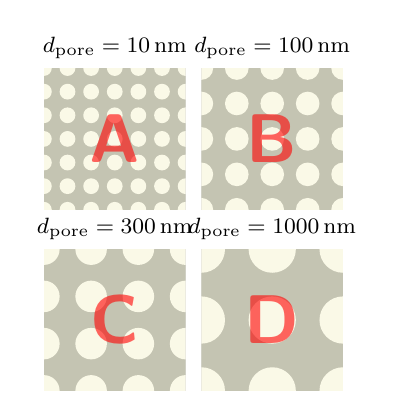
\begin{tikzpicture}
    \tikzset{%
        pics/dpore/.style args={#1/#2/#3/#4}{code={%
                        \tikzmath{%
                            \dpore=#1;
                            \deltafig=1.8;
                            \numpore=#2;
                            \deltawall=(\deltafig-\numpore*\dpore)/\numpore;
                        };

                        \begin{scope}
                            \clip (0, 0) rectangle ++(\deltafig, \deltafig);
                            \fill [GDLcolor] (0, 0) rectangle ++(\deltafig, \deltafig);
                            \foreach \i in {0, ..., \numpore} {%
                                    \foreach \j in {0, ..., \numpore} {%
                                            \fill [white] ({\i*(\dpore+\deltawall)}, {\j*(\dpore+\deltawall)}) circle (\dpore);
                                        }
                                };
                            \fill [ELcolor, opacity=0.4] (0, 0) rectangle ++(\deltafig, \deltafig);
                        \end{scope}

                        \node at (\deltafig/2, \deltafig) [above] {\fontsize{8pt}{0pt}\selectfont\ensuremath{d_\mathrm{pore} = \qty{#3}{\nm}}};
                        \node at (\deltafig/2, \deltafig/2) [opacity=0.6] {\sffamily\bfseries\color{red}\fontsize{30pt}{30pt}\selectfont #4};
                    }
            }
    }

    % dpore/numpore/dpore text/A
    \pic at (0, 0) {dpore=0.1/6/10/A};
    \pic at (2, 0) {dpore=0.15/4/100/B};
    \pic at (0, -2.3) {dpore=0.2/3/300/C};
    \pic at (2, -2.3) {dpore=0.3/2/1000/D};
\end{tikzpicture}
\end{document}